%% *************************************************************************
%%
%% This is the PDD for Rovers 2018
%%
%% This document uses IEEEtran.cls, the official IEEE LaTeX class
%% for authors of the Institute of Electrical and Electronics Engineers
%% (IEEE) Transactions journals and conferences.
%%
%% *************************************************************************

\documentclass[conference]{IEEEtran} % http://www.ctan.org/pkg/ieeetran
 \usepackage{ltxtable, tabularx, longtable} 
\usepackage{tabularx} % fix tables
  \newcolumntype{L}{>{\raggedright\arraybackslash}X}   
\usepackage{multirow}  
\usepackage{blindtext} % enable placeholder text generator
\usepackage{graphicx} % enable toolbox for embedding figures and pictures
\usepackage{nomencl} % enable package for adding a list of variables and constants at the beginning, aka "nomenclature"
\usepackage{siunitx} % enable package for easily formatting units
\usepackage{hyperref} % enable package for cross-referencing figures, sections, references etc.
% how to use hyperref: http://www2.washjeff.edu/users/rhigginbottom/latex/resources/lecture09.pdf
\usepackage[T1]{fontenc} % change text encoding to make it more crisp
\usepackage{etoolbox} % enable conditionals for help text
\usepackage{booktabs} % make beautiful tables!
\usepackage[utf8]{inputenc}
\usepackage[english]{babel}
 
\usepackage{hyperref}
\hypersetup{
    colorlinks=true,
    linkcolor=blue,
    filecolor=magenta,      
    urlcolor=cyan,
}

% initialize nomenclature package
\makenomenclature{}

% set title. choose something as descriptive and precise as possible. Descriptive > sounding cool. remember this!
\title{Rovers} %TODO come up with a better title

\author{
  \IEEEauthorblockN{Thomas~Hall\IEEEauthorrefmark{1}}
  \IEEEauthorblockA{RIT Space Exploration, Rochester Institute of Technology \\ Rochester, N.Y. \\ Email: \IEEEauthorrefmark{1}tjh2822@g.rit.edu }
}

% page header for pages other than cover page
\markboth{Project Design Document Standard}%
{Hall \MakeLowercase{\textit{et al.}}: RIT Space Exploration}

\begin{document}
\maketitle
\hyphenation{explor-ation}

\begin{abstract}
Design and construction of a mock-rover. 
The goal of this project is delivering a functioning mock rover.
We define mock rover as a functioning rover built to specifications for a mock mission as it will not be launched.
A rover would be an area of space exploration completely new to RIT SPEX, because of this there are a lot of unknowns that need to be answered before starting this project. 
Because of this the project will require a large amount of prototyping and testing. 
The team would look at the talent and skills of RIT Space Exploration and answer the question: what caliber of rover are we able to make. 
It would employ a multidisciplinary team for construction and development. The project would be slated to run for two semesters. 
The rover would be extremely promotable and would look great at Imagine RIT. 
\end{abstract}

\label{sec:nomenclature}
\newcommand{\nomunit}[1]{\renewcommand{\nomentryend}{\hspace*{\fill}#1}}
\renewcommand{\nompreamble}{}

\nomenclature{RIT}{Rochester Institute of Technology}
\nomenclature{SPEX}{RIT Space Exploration}
\nomenclature{PDD}{Project Design Document}
\nomenclature{URC}{University Robotics Competition}
\nomenclature{MVP}{Minimum Viable Product}

% Intro
\section{Introduction}
\label{sec:introduction}

\IEEEPARstart{R}{obotics}  and by extension rovers are a tremendously important
part of space exploration. 
This is also an area that RIT Space Exploration has very little experience with project-wise.
The purpose of this project is to assess and assert the capability of RIT SPEX regarding the construction and fabrication of a mock-rover and then begin construction. 
As this is a new area to RIT SPEX, prototyping and experimenting is necessary to most effectively accomplish this goal. 
This project will look at the unknowns, technical challenges, project management, and member skills of RIT Space Exploration in regard to a University Rover Competition (URC) capable rover and rover construction. 
The URC is hosted by The Mars Society annually. 
It is very competitive and requires a very complex and expensive rover that is currently out of scope for SPEX. 
This rover would need to be capable of full autonomous navigation, soil collection and analysis, and precise robotics. 
This project is the first step in building the skills for such a team.
Rovers are important, they are one of the primary ways we explore space and other planets. 
This project exists to get our members experience with rovers by building such a rover. 

\section{Primary Objective}
\label{sec:primary-obj}
The goal of this project is delivering a functioning mock rover.
We define mock rover as a functioning rover built to specifications for a mock mission as it will not be launched. 
We define rover as a vehicle for driving over rough terrain, especially one driven by remote control.
The rover will allow the team to develop skills and knowledge to build a
more feature completer rover in the future. 
These skills include rover fabrication and design, autonomous navigation, electrical system design, rover testing, computer vision, and robotics.
The rover will be testing using events designed like the URC but scaled down to fit the scope of this rover. 
We will be using time as a metric as well as binary metrics for completion of the parts of the competition. 
Some features might behave differently than expected or planned these features will be evaluated accordingly.
This includes ’does the rocker-bogie system works as intended’, ’will the rover stop when directed at an obstacle’, etc. 
The details are defined in the minimum viable product section.

\subsection{Minimum Viable Product}
\label{subsec:mvp}
The minimum viable product (MVP) has been defined by the basics of what can be called a 'functioning rover'. This includes features like suspension, motors, power and controls. The MVP is defined by the following features: 

\begin{table}[hb!]
    \caption{Minimum Viable Product}
    \centering
    {\renewcommand{\arraystretch}{1.5}
    \begin{tabularx}{\linewidth}{LL} 
    \hline
    \textbf{Feature} & \textbf{Reason} \\
    \hline
    Rocker-bogie-like suspension & This is the NASA preferred rover suspension style. \\
    Ability to control remotely (such as a gamepad) & Remote control is essential for rovers. \\
    Ability to traverse terrain such as gravel, cement, and asphalt & Multi-terrain traversal is important for rovers. \\
    Technical report on GitHub & This will allow for future teams to easily learn from this teams experience. \\
    Rover hardware & Having a physical rover is important for a rover project as it allows for lessons to be learned in construction. \\ 
    Present at Imagine RIT & This is essential for promotional value. \\
    Partial self-driving & Partially autonomous navigation for future URC readiness. \\
    \hline
    \end{tabularx}
    }
\label{tab:mvp-one}
\end{table}

\subsection{Improvements}
\label{subsec:improvements}
The MVP is intended to be flexible in implementation depending on funding. 
The purpose of the project is to gain experience in rovers and robotics and this can be done in a number of form factors.
The size and materials are not defined because of this. 
Should the funding allow for it there are many improvements that can be made beyond the MVP. 
This allows for more experience to be gained, thus fulfilling the goals of the project.

\begin{table}[ht!]
    \caption{Improvements}
    \centering
    {\renewcommand{\arraystretch}{1.5}
    \begin{tabularx}{\linewidth}{LL}
    \hline
    \textbf{Feature} & \textbf{Reason} \\  
    \hline
    Lidar based CV & Autonomous navigation for future URC readiness. \\
    Improved navigation with use of GPS system & Additional navigation options. \\
    Robotic arm with 3+ degrees of freedom & URC readiness and rover capabilities. \\ 
    Drill or grasper attachment & Increased capabilities of the robotic arm. \\
    Soil sample analysis with Archimedes' screw & Scientific possibilities. \\
    Larger and or faster rover & Able to traverse obstacles of greater magnitude or hold more scientific equipment for future expansion. \\
    Solar cells & Additional long-term navigation viability and experience. \\
    Web control interface with GUI & Easier navigation. \\
    Durable construction & Carbon fiber or similar materials for long term viability. \\
    On board batteries & Lithium Ion, 18650s or similar battery technology for remote abilities. \\
    Long range communications & Ability to communicate with the rover at lengths of up to one kilometer allows for URC readiness. \\
    \hline
    \end{tabularx}
    }
\label{tab:mvp-two}
\end{table}

\section{Secondary Objectives}
\label{sec:secondary-obj}
The study will also investigate the University Rover Competition (URC) as hosted by the Mars Society as a potential long term goal. 
The team will accomplish this by evaluating how many of the MVP improvements are accomplished. 
If none of these improvements are able to be implemented then the team is not near URC ready.
The competition is held annually and features four very intense competitions. 
Such a rover would need to be fully self navigating, perform scientific analysis on soil samples, and having a robotic arm capable of fine motor control. 
Such a project would be among the most ambitious SPEX has ever attempted. 
These features line up with the improvements section of the MVP.
The skills learned from this project should be applicable to such a future project. 
This secondary objective is directly related to the long-term vision of the rover project. 

\section{Benefit to SPEX}
\label{sec:benefit}

\subsection{Space Exploration}
\label{subsec:spacex}
Rovers are a huge part of space exploration. 
There are eight active missions on Mars. 
Four of those include rovers. 
To ignore this fact would be to ignore a large part of space exploration.
Currently RIT SPEX is not involved with rovers.
It would be beneficial to our members to get some experience in this area.

\subsection{Promotions and Funding}
\label{subsec:promos}
A rover would be a popular demonstration at ImagineRIT.
The rover would be rather large and would attract many eyes. 
We could even demo it outside if there is sufficient space. 
A rover would be very easy to get video and photos of for SPEX promotions. 
Having a rover is also another opportunity for SPEX to fundraise. 
There is plenty of space to place company logos on the body of the rover. 
It would also allow for SPEX to reach out to robotics companies.

\subsection{Computer Science}
\label{subsec:cs}
\subsubsection{Member Retention and Expansion}
\label{subsubsec:cs}
The potential self-driving component would be the heaviest computer science project SPEX would have attempted, this would help with retention of CS and SE majors. 
There are many features included in the MVP that require significant computer science skills as well.
This includes navigation, power management, communications and more.
That will give computing-related majors another option for SPEX involvement, also helping retention.

\subsubsection{Artificial Intelligence}
\label{subsubsec:ai}
Some of the potential self-driving features will likely be implemented with artificial intelligence. In particular the fully autonomous navigation would require this.
Machine learning and artificial intelligence are at the forefront of computer science right now. 
They are heavily desired in industry, including space exploration.
There are limited options for RIT students to get involved with AI project wise, this can help with that. 
There is another AI-based student group (RITficial Intelligence) on campus that has members interested in these projects but the group lacks the funding to start any.
RIT SPEX could partner with this group to recruit talent.

\subsection{Robotics}
\label{subsec:robotics}
Robotics are also a heavily desired area in the space industry. 
Currently RIT SPEX does not have any projects with robotics as a focus. 
Robotics is also a potential area for collaboration with faculty as there are RIT faculty that are investigating this area.
RIT is host to the FIRST robotics competition which would be a good source to get information and help from. 
However, most university students volunteer to run this competition instead of participating. 
This competition is at the high school level and many students want an opportunity to do something more advanced. 
SPEX could even show off the rover at the FIRST robotics competition (especially if the rover competed in the University Robotics Competition or a similar competition). 
RIT would love the promotional value an it would be a great recruitment and fundraising opportunity for RIT SPEX.

\subsection{Challenge}
\label{subsec:challenge}
The project including just a few of the improvements would be very ambitious. 
It would require at a minimum a handful (4-5) members each with different areas of expertise just for the MVP.
The team would have to be even larger to accommodate some of the improvements as a larger team would be able to accomplish more. 
Aside from technical skills, members would need to be knowledge in \LaTeX{}, documentation, notetaking, and good research practices. 
Challenging projects allow for members to gain even more experience. 

\subsection{Documentation}
\label{subsec:docs}
It is important that the team members document the sources they use to gather information. 
There will be a Google Drive folder that will hold notes with links to any books, articles, media or their sources that are relevant to the rover project. 
The software and hardware will be tracked on GitHub (including the technical report).
One of the areas SPEX is currently struggling with is knowledge transfer.
This project should serve as an example to other SPEX projects on how information should be passed on from year to year.
Being able to successfully transfer knowledge from year to year will greatly advance the ability for RIT SPEX to complete more ambitious projects.

\subsection{Project Management Skills}
\label{subsec:project-management}
The purpose of this project is to investigate and implement a mock rover.
Because of this the team members must be in the mindset to analyze each part of the project and identify as many problem areas that need answers as possible. 
This means being specific on how we are going to accomplish our goals.
We want our team asking the question:"what material, what algorithm, with what method will we be accomplishing this?"
It is very easy to over estimate the team's ability especially when the project is so new to the team.
These are skills that benefit RIT SPEX. 

\section{Implementation}
\label{sec:implementation}
This project would involve divvying out the different project areas to the different team members or small groups and each week meeting to discuss progress.
The rover project lends itself well to modularity.
This will allow us to set up the project in a way that best matches the skillset of the team we have. 
The team would take this information, refine it and put it into the technical report along with construction. 

\subsection{Deliverables}
\label{subsec:deliverables}
The deliverable includes the technical report, rover software, and rover hardware.
The primary deliverables of this project will be the technical report and the rover itself by the end of the second semester.
It is also noted that the materials that the team will come across or notes should also be saved in an Google Drive folder for future reference. 
The team will also present at SPEX design reviews and the weekly checkups at general meetings with the areas the team members are working on that week.
The project is intended to last 2 semesters with the deliverable of a mock rover and a technical report.   

\subsubsection{Technical Report}
\label{techreport}
The technical report of the rover is a design document complete with the hardware, software, and electrical components of the rover. 
This report is important as it allows for a future team to easily learn from the past team's experience. 
This Technical Report will be hosted on GitHub. 
This will also include the results of the rover tests and the teams recommendations based on them. 

\subsubsection{Rover Software}
\label{roversoftware}
The rover software has to be written and hosted on GitHub. 
This will include rover features such as navigation, control, and power regulation. 
The rover need to be controlled so software must be made to do so. 
This means the rover electronics must be integrated with a control application. 
The rover will need to distribute power to the motors in the wheels so software will need to be made to regulate such power. 
There will also need to be software for the autonomous or partially autonomous features on the rover. 

\subsubsection{Rover Hardware}
\label{roverhardware}
The rover will need to be constructed and tested. Because of this a physically constructed rover is needed. This will be necessary for ImagineRIT for cool factor. This includes the rover body, mast, suspension, and wheels. 

\begin{figure}[hb!]
  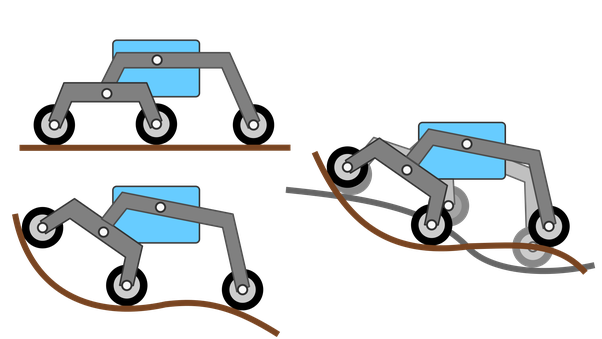
\includegraphics[width=\linewidth]{figs/rocker-bogie.png}
  \caption{Rocker-Bogie mechanism}
\label{fig:rockerbogie}
\end{figure}

\subsection{Milestones}
\label{subsec:milestones}
The largest milestones for the technical report would be the would be draft and completion. 
The rover itself would include the various CAD models of the rover, software milestones, electrical system completion, and drive train system. 
Other milestones include securing funding and completion of the learning period at the beginning of the fall semester.
The improvements would be developed in tandem with the MVP, however the MVP will always come first. 
The improvements will attempted only if there is funding and members to spare. 
The improvements are varied in complexity and some would take more time than others. 
Each improvement would be on its own timeline with milestones along with the funding.
However the team will try to be proactive with funding and always stay a little ahead so improvements can be started right away.

\begin{table}[ht!]
    \caption{Timeline}
    \centering
    {\renewcommand{\arraystretch}{1.5}
    \begin{tabularx}{\linewidth}{LL} 
    \hline
    \textbf{Time} & \textbf{Phase} \\
    \hline
    August & Learning and Planning Phase \\
    September - November & Design Phase  \\
    December - February & Manufacturing Phase \\
    March - May & Testing Phase \\
    \hline
    \end{tabularx}
    }
\label{tab:timeline}
\end{table}

\subsubsection{Learning and Planning Phase}
\label{subsubsec:phaseone}
Learn about rovers and create a set of plans to help guide the team through the execution and closure phases of the project. Requirements that are associated with a project result are specified as clearly as possible.
\subsubsection{Design Phase}
\label{subsubsec:phasetwo}
Designs are developed, with which the project result can apparently be achieved. Depending on the subject of the project, the products of the design phase can include dioramas, sketches, flow charts, site trees, HTML screen designs, prototypes, photo impressions, UML schemas, and CAD models created.
\subsubsection{Manufacturing and Construction Phase}
\label{subsubsec:phasethree}
Construction of the actual project result. Programmers are occupied with encoding, engineers are machining and building, the actual reorganization takes place.
\subsubsection{Testing Phase}
\label{subsubsec:phasefour}
Formally controlled and focused testing is performed to uncover errors and bugs in the IT solution that need to be resolved. This includes software unit testing and a mock URC-like competition. 

\section{Externalities}
\label{sec:externalities}
\subsection{Prerequisite Skills}
\label{subsec:skills}
The project is going to require members that are knowledgeable in mechanical design and manufacturing, software engineering, (potentially) machine learning, electrical engineering, and project management. 
These members will also need to be experienced in research and design document work. 
Though this seems simple, finding SPEX members to do this well may be a challenge due to competition from other projects. 
Building a rover, especially one built to URC specifications requires a large team with a diverse set of technical skills. 
This project will require SPEX to look at and asses what areas are sufficient and what areas need to be developed in order to build a rover. 
It will also let us know to what spec we are currently capable of building such a rover. 

\subsection{Funding Requirements}
\label{subsec:funding}
The rover project is looking at a minimal funding amount of \$500.00 USD from RIT SPEX. This funding is needed to make a rover that fulfills the MVP defined in the Primary Objective section. In order to give a better deliverable the team will also be reaching out to a large list of companies looking for further funding through sponsorship. 
Increasing the funding to \$2500.00 USD would allow for the team to construct a more feature complete rover. Components like LIDAR sensors and long-range remote communications are expensive. 
Though a rover can be made without them additional funding allows for the rover project to expand in scope. 
We are aiming for the \$2500.00 price point to achieve the MVP as well as improvements like extended battery, Lidar, communications and improved navigation. There are some improvements that can be made under the \$500.00 price point including the advanced navigation station and partial autonomy. 
However, it is noteworthy that the project is flexible enough to function on various amounts of funding as long as it is above the \$500.00 price point.

\subsection{Faculty Support}
\label{subsec:faculty}
Support from faculty could greatly advance this study and what RIT SPEX is capable robotics wise. 
It is not necessary but would be very helpful. 
Professors could help with funding, rover design, hardware selection and general advice. 
Rovers and robotics are new to SPEX and someone with experience could help this. 
The team should reach out to professors for advice and help. 
There are many professors at RIT with interest in robotics or computer vision. 
With some recommendations from SPEX alumni we have a short list of professors who might be interested. 
There is also a large robotics competition which is hosted yearly at RIT, FIRST robotics. 
This is also a potential source of support from RIT faculty. 

\begin{table}[ht!]
    \caption{Potential Faculty Support}
    \centering
    {\renewcommand{\arraystretch}{1.5}
    \begin{tabularx}{\linewidth}{LLL} 
    \hline
    \textbf{Professor} & \textbf{Department / Field} & \textbf{Email Address} \\
    \hline
    Dr. Ugur Sahin & Mathematics (Researches Computer Vision) & us-grd@cs.rit.edu \\
    Dr Ferat Sahin & KGCOE (Robotics) & feseee@rit.edu \\
    \hline
    \end{tabularx}
    }
\label{tab:fac-sup}
\end{table}

\subsection{Long-Term Vision}
\label{subsec:vision}
The long-term vision of this project is to open RIT Space Exploration up to a new area of projects and development. 
Robotics and rovers are at the core of deep space exploration and most science missions. 
The project is also intended to lead into a future rover project with expanded capabilities.
The University Rover Challenge is hosted by the Mars Society. 
It features very competitive and expensive rovers. 
These rovers feature autonomous navigation, fine control robotics, scientific drill and more. 
It is a worthy long term goal. 

\section*{Acknowledgements}
The author would like to thank SPEX alumni Phil Linden for creating the PDD template, SPEX alumni 'TJ' Tarazevits for feedback on project design and management, SPEX alumni Daniel Mitchell and Matthew Glazer for their feedback on electrical system design, Anthony Hennig for founding RIT Space Exploration, and all the SPEX members that continue to invest their time and energy into the pursuit of space exploration. 

\section{References}
\begin{itemize}
  \item \href{http://urc.marssociety.org/files/University%20Rover%20Challenge%20Rules%202018.pdf}{University Rover Challenge Download the Requirements and Guidelines PDF}
  \item \href{http://urc.marssociety.org/home/q-a}{RC2018 Q\&A}
\end{itemize}
\onecolumn
\appendices{}

\end{document}
